\documentclass[a4paper, oneside]{article} 
\usepackage{tikz}
\usepackage{amsmath}
\usepackage{amsthm}
\usepackage{amssymb}
\usepackage{graphicx}
\usepackage[hidelinks]{hyperref}
\usepackage{enumitem}
\usepackage{nicefrac}
\usepackage{empheq}
\usepackage{xcolor}
\usepackage{array}
\usepackage{indentfirst}
\usepackage{caption}
\usepackage{subcaption}
\usepackage{enumitem}
\usepackage[fancysections, titlepage, pagenumber]{polytechnique}
\usepackage{float}

\theoremstyle{plain}
\newtheorem{theorem}{Theorem}
\setcounter{tocdepth}{2}

\newcommand{\castle}{C{\small.}A{\small.}S{\small.}T{\small.}L{\small.}E{\small.}}

\title[\castle{}]{Market Design Project: C.A.S.T.L.E.}
\subtitle{Capacity-Aligned Stable Teaching Location Engine\\
Tackling classroom allocation in Universities}
\author{Matthieu MINGUET}
\date{December 2024}

\begin{document}
\maketitle

\phantomsection
\section*{Executive Summary}
\addcontentsline{toc}{section}{Executive Summary}
The allocation of classrooms in universities represents a complex challenge that currently relies on manual processes and basic criteria like class size, 
leading to inefficiencies and suboptimal matching between courses and rooms. 

This project presents \castle{} (Capacity-Aligned Stable Teaching Location Engine), a market design mechanism that automates classroom allocation through efficient preference matching.
It achieves this through a modified Deferred Acceptance algorithm that matches courses to room types (one to many matching) based on stated preferences while ensuring capacity constraints are met.
Key features and results include:

\begin{itemize}
	\item Theoretical guarantees of stability and Pareto efficiency within room types, and limited manipulability encouraging honest preference reporting
	\item Computational efficiency with $O(\text{number of courses}\cdot \text{number of rooms})$ average-case complexity (milliseconds for typical medium size university scenarios)
	\item High performance in simulations: $>95\%$ allocation rate with over a large proportion of courses matched to top preferences.
	\item Empirical validation of preferences existence and compatibility with the system through surveys at École Polytechnique.
	\item Maximization of the utilization of most-requested rooms in terms of use ($100\%$), and capacity ($>80\%$).
	\item Minimal faculty input required: 6 ranked preferences sufficient for optimal results, and rare fringe cases requiring manual intervention.
\end{itemize}

The system represents a significant improvement over current manual allocation methods, offering a scalable, transparent solution that could benefit over 5,000 universities worldwide. 
\castle{}'s modular design allows for customization to specific needs while maintaining its core properties. This system is much needed, easy to use and deploy, and has
very good market design properties.
\pagebreak

\tableofcontents
\pagebreak

\phantomsection
\section*{Introduction}
\addcontentsline{toc}{section}{Introduction}

The idea for this project came from a simple yet telling experience: a professor struggling at the front of a classroom, trying to juggle between a whiteboard
and a projector screen that can't be used simultaneously. In the meantime, I think back to my physics professor in \textit{Classe Préparatoire} who would advocate
for a traditional blackboard and chalk over anything else. These contrasting needs highlight a fundamental challenge in academic institution: different 
courses and teaching styles require different classroom environments.\\

The inefficiencies in current room allocation systems become apparent when observing these frictions. But beyond teaching tools, the geographical location of the room
relative to both students and faculty, proximity to amenities, and layout impact the teaching and learning experience.\\

These observations point to a deeper market design challenge: how can we efficiently match courses to classrooms while accounting for diverse preferences, 
physical constraints, and institutional requirements? Current allocation systems, typically managed through manual spreadsheets or basic scheduling software, 
fail to capture these nuanced preferences and often result in suboptimal matches. The challenge is further complicated by the expanding size and complexity of 
modern universities, with multiple programs competing for limited space resources.\\

This project proposes a novel solution to this problem: \castle{}, a matching mechanism that aims to apply 
market design principles to create more efficient and satisfying matches between courses and classrooms, while ensuring its ease of use and deployment.\\

We will first \textbf{analyze the current systems} in place at Ecole Polytechnique and Clermont School of Business, identifying their flaws and limitations, then doing a market sizing and
reviewing the leading academic paper on the subject. Then, we will \textbf{present the core principles} of \castle{}, the matching algorithm implemented, and its properties. 
Finally, we will detail the \textbf{implementation and testing} of the algorithm, and the results of a pilot study at Ecole Polytechnique.\\
\pagebreak

\section{Due Diligence}
\subsection{Current System at Ecole Polytechnique}
X currently operates a centralized room allocation system managed by the Registrar's office through a shared spreadsheet.
While the basic objective of assigning rooms to all classes is met, the system faces significant operational challenges.
The manual allocation process is time-consuming, requires frequent bargaining between departments, and often fails to meet teacher preferences and specific classroom needs.
Moreover, it does not provide a reporting of what the faculty values for their classrooms.\\

The system's current stability relies heavily on the natural distribution of class sizes, particularly in the \textit{Cycle Ingénieur} program where enrollment decreases
from 550 students in first year to increasingly smaller specialized groups through second and third year. This pattern allows for predictable allocations, such as Poincare for large
lectures and smaller rooms for tutorials, especially when third-year students are off-campus. With the inversion of tutorials and lectures times based on the year, the system can support
the needs of the program.

However, mounting pressure from expanding masters and bachelor programs is straining this delicate balance. The competition for rooms,
especially between second and third-year needs, is intensifying. While the system functions now due to fortunate enrollment patterns,
it lacks the robustness to handle future growth and increasing complexity.

\subsubsection{Flaws in the current system}
In terms of market design, this system is a centralized dictatorship, as in a control economy where resources are allocated based on the sole criteria of class size. It's flaws which we will detail in the following table:\\

\begin{tabular}{|p{2.5cm}|p{10cm}|>{\centering\arraybackslash}p{2.5cm}|}
	\hline
	\textbf{Flaw}                                                                                  & \textbf{Description} & \textbf{Intensity} \\
	\hline
	Information Problem                                                                            &
	\begin{itemize}[leftmargin=*,nosep,topsep=0pt,partopsep=0pt,before=\vspace{-\baselineskip}]
		\item No preference elicitation
		\item Manual spreadsheet means no way to communicate preferences, constraints, or trade
	\end{itemize}  &
	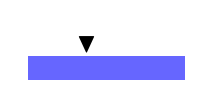
\begin{tikzpicture}
		\fill[blue!60] (0,0) rectangle (2,0.3);
		\node[anchor=center] at (0.75,0.45) {$\blacktriangledown$};
	\end{tikzpicture}                                                                                 \\[2ex]
	\hline
	Matching Mechanism                                                                             &
	\begin{itemize}[leftmargin=*,nosep,topsep=0pt,partopsep=0pt,before=\vspace{-\baselineskip}]
		\item Single-Criterion Optimization: capacity matching
		\item Manual Coordination Cost: bargaining
		\item No formal Trading Mechanism: no beneficial trades
	\end{itemize}  &
	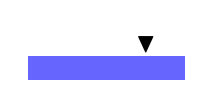
\begin{tikzpicture}
		\fill[blue!60] (0,0) rectangle (2,0.3);
		\node[anchor=center] at (1.5,0.45) {$\blacktriangledown$};
	\end{tikzpicture}                                                                                  \\[2ex]
	\hline
	Incentive Problems                                                                             &
	\begin{itemize}[leftmargin=*,nosep,topsep=0pt,partopsep=0pt,before=\vspace{-\baselineskip}]
		\item No strategic reporting: no formal way to express the preferences for rooms or features
		\item Lack of Price Mechanism: no way of quantifying preferences
	\end{itemize}  &
	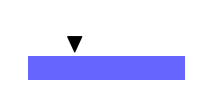
\begin{tikzpicture}
		\fill[blue!60] (0,0) rectangle (2,0.3);
		\node[anchor=center] at (0.6,0.45) {$\blacktriangledown$};
	\end{tikzpicture}                                                                                  \\[2ex]
	\hline
	Scalability                                                                                    &
	\begin{itemize}[leftmargin=*,nosep,topsep=0pt,partopsep=0pt,before=\vspace{-\baselineskip}]
		\item Brittle equilibrium: program change or growth could pose a threat to the current system
		\item Manual processing bottleneck
	\end{itemize} &
	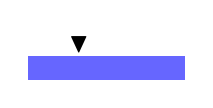
\begin{tikzpicture}
		\fill[blue!60] (0,0) rectangle (2,0.3);
		\node[anchor=center] at (0.65,0.45) {$\blacktriangledown$};
	\end{tikzpicture}                                                                                 \\[2ex]
	\hline
	Efficiency problem                                                                             &
	\begin{itemize}[leftmargin=*,nosep,topsep=0pt,partopsep=0pt,before=\vspace{-\baselineskip}]
		\item No Optimization Algorithm
		\item Suboptimal Outcomes: room for Pareto improvements
		\item Resource Utilization: inefficient use of features and capabilities
	\end{itemize} &
	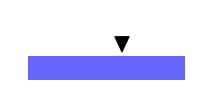
\begin{tikzpicture}
		\fill[blue!60] (0,0) rectangle (2,0.3);
		\node[anchor=center] at (1.2,0.45) {$\blacktriangledown$};
	\end{tikzpicture}                                                                                  \\[2ex]
	\hline
	Adaptation and flexibility                                                                     &
	\begin{itemize}[leftmargin=*,nosep,topsep=0pt,partopsep=0pt,before=\vspace{-\baselineskip}]
		\item Rigid system: changes mid-term can be difficult
		\item Limited feedback loop: for allocation and features
	\end{itemize} &
	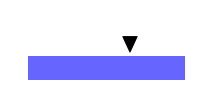
\begin{tikzpicture}
		\fill[blue!60] (0,0) rectangle (2,0.3);
		\node[anchor=center] at (1.3,0.45) {$\blacktriangledown$};
	\end{tikzpicture}                                                                                  \\[2ex]
	\hline
\end{tabular}
\linebreak

\vspace{0.05cm}

As we can see, while the current system has major flaws like the lack of a matching mechanism,
it still ensures all teachers have a room, and the school has functioned with this system for the past few years without any issues,
especially when the \textit{Cycle Ingénieur} program was the only program at the school.

\subsection{Current system at Clermont School of Business (Clermont SB)}
The Clermont SB has a similar system to Ecole Polytechnique, with a centralized room allocation and planning system. A dedicated member of staff is responsible
for managing the system in place: Program Directors submit room requirement and planning forms to the Planning Office, which then manually attributes the rooms based on the information provided,
and the availabilities of the rooms. These types of requirements include the number of rooms, the equipment, expected cohort size, and if the rooms need to be close to each other or not (for example for group work).
The number of variables makes it very difficult to find a solution satisfying all requirements of all courses.
While the system allows for inputs from the faculty, the major issue si that the large number of programs and the increasing number of students in each program
is making the system increasingly complex to manage by hand and is leading to inefficiencies and tensions in the allocation. Moreover, this system is quite slow and requires
a large amount of time to manage, which could be streamlined and better used elsewhere. Finally, the system is not transparent,
and the faculty does not have a clear understanding of how the rooms are allocated, while it also doesn't encourage truthful reporting of preferences.

\subsubsection{Flaws in the current system}
Similarly as what we did for Ecole Polytechnique, we have identified the following flaws in the current system at Clermont SB:\\

\begin{tabular}{|p{2.5cm}|p{10cm}|>{\centering\arraybackslash}p{2.5cm}|}
	\hline
	\textbf{Flaw}                                                                                  & \textbf{Description} & \textbf{Intensity} \\
	\hline
	Information Problem                                                                            &
	\begin{itemize}[leftmargin=*,nosep,topsep=0pt,partopsep=0pt,before=\vspace{-\baselineskip}]
		\item Preference reporting through requirement forms
		\item Lack of transparency in allocation process
	\end{itemize} &
	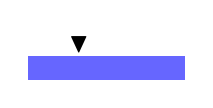
\begin{tikzpicture}
		\fill[blue!60] (0,0) rectangle (2,0.3);
		\node[anchor=center] at (0.65,0.45) {$\blacktriangledown$};
	\end{tikzpicture}                                                                                 \\[2ex]
	\hline
	Matching Mechanism                                                                             &
	\begin{itemize}[leftmargin=*,nosep,topsep=0pt,partopsep=0pt,before=\vspace{-\baselineskip}]
		\item Manual attribution based on submitted forms
		\item Single-person decision making process
		\item No formal mechanism for resolving conflicts
	\end{itemize} &
	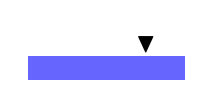
\begin{tikzpicture}
		\fill[blue!60] (0,0) rectangle (2,0.3);
		\node[anchor=center] at (1.5,0.45) {$\blacktriangledown$};
	\end{tikzpicture}                                                                                  \\[2ex]
	\hline
	Incentive Problems                                                                             &
	\begin{itemize}[leftmargin=*,nosep,topsep=0pt,partopsep=0pt,before=\vspace{-\baselineskip}]
		\item No incentive for truthful preference reporting
		\item Lack of feedback mechanism
	\end{itemize} &
	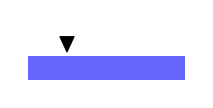
\begin{tikzpicture}
		\fill[blue!60] (0,0) rectangle (2,0.3);
		\node[anchor=center] at (0.5,0.45) {$\blacktriangledown$};
	\end{tikzpicture}                                                                                  \\[2ex]
	\hline
	Scalability                                                                                    &
	\begin{itemize}[leftmargin=*,nosep,topsep=0pt,partopsep=0pt,before=\vspace{-\baselineskip}]
		\item Growing complexity with increasing programs
		\item Rising student numbers strain current system
		\item Single point of failure (dedicated staff member)
	\end{itemize} &
	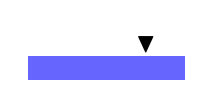
\begin{tikzpicture}
		\fill[blue!60] (0,0) rectangle (2,0.3);
		\node[anchor=center] at (1.5,0.45) {$\blacktriangledown$};
	\end{tikzpicture}                                                                                  \\[2ex]
	\hline
	Efficiency problem                                                                             &
	\begin{itemize}[leftmargin=*,nosep,topsep=0pt,partopsep=0pt,before=\vspace{-\baselineskip}]
		\item Time-intensive manual process
		\item Inefficiencies in allocation
		\item Resource under-utilization due to information gaps
	\end{itemize} &
	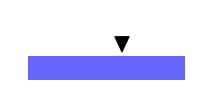
\begin{tikzpicture}
		\fill[blue!60] (0,0) rectangle (2,0.3);
		\node[anchor=center] at (1.2,0.45) {$\blacktriangledown$};
	\end{tikzpicture}                                                                                  \\[2ex]
	\hline
	Adaptation and flexibility                                                                     &
	\begin{itemize}[leftmargin=*,nosep,topsep=0pt,partopsep=0pt,before=\vspace{-\baselineskip}]
		\item System struggles with program diversity
		\item Difficult to make mid-term adjustments
		\item Slow response to changing needs
	\end{itemize} &
	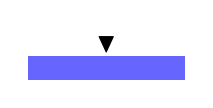
\begin{tikzpicture}
		\fill[blue!60] (0,0) rectangle (2,0.3);
		\node[anchor=center] at (1,0.45) {$\blacktriangledown$};
	\end{tikzpicture}                                                                                    \\[2ex]
	\hline
\end{tabular}
\linebreak

As we can see, while this system offers more inputs from the different stakeholders, it is limited by the fact that it has to be
manually run, and an increasing number of programs and students compared to the number of rooms, or even more rooms could cause issues
regarding the length of the process and the fairness of the allocation.

\subsection{Market Sizing and existing solutions}
\subsubsection{Market Sizing}
There are around $18500$ universities worldwide, representing around $250$m students. However, a new system such as \castle{} would be more suited to larger universities, especially in developed countries, where the number of students is higher, and programs are more diverse.
As such, we estimate a theoretical market size of $5000$ universities, mainly in Europe and North America.
At first, this system would target around 80 universities in these markets, which considering their size could already impact upwards of $200000$ students.
Thus, \castle{} could bring an improvement over the current systems in place in these universities, and potentially be a game-changer in the way universities allocate their resources.

\subsubsection{Existing Papers}
Classroom allocation or time-tabling is a well-studied problem in the literature, with many papers proposing different solutions to the problem.
For example, Rivero, Escárcega, and Velasco (2021) proposed an Integer Linear Programming model for classroom assignment to tackle this issue, while other solutions
focus on graph coloring algorithms or genetic algorithms to allocate classrooms and timetables. In almost all cases, the solution to solve both
timetabling and classroom allocation is to decouple the two problems and solve them sequentially, as the classroom allocation algorithm generally output near 100\% utilization of the rooms,
which we will see is also the case for \castle{}.
The basic formulation of the problem for classroom allocation is as follows:
\begin{itemize}
	\item Let $x_{ij}$ be a binary variable where $i$ the classroom, $j$ the course and : $x_{ij} = 1$ if course $j$ is assigned to classroom $i$, $0$ otherwise.
	\item The objective function is : $\min \sum_{i,j} c_{ij}x_{ij}$ where $c_{ij}$ is the cost of assigning course $j$ to classroom $i$.
	\item $c_{ij}$ represents the cost of assigning class $j$ to classroom $i$, and can incorporate functions like room size mismatch, distance from the professor's department, equipment mismatch, etc.
\end{itemize}
The constraints are generally the following:
\begin{itemize}
	\item Single assignment constraint: $\sum_{i} x_{ij} = 1$ for all $j$
	\item Room capacity constraint: $\text{enrollment}_j \leq \text{capacity}_i \forall x_{ij} = 1$
\end{itemize}
In cases where timetables are also considered, the time $t$ is added as a third dimension to the problem, and the constraints are modified to include the time dimension (professor, room and student availabilities)
This formulation guarantees an optimal solution (if solvable) and is able to balance different objectives by weighting the $c_{ij}$, while being very flexible in terms of constraints and objectives.\\

However it is an NP-hard problem to solve and the solution space grows exponentially with the number of rooms, classes (and time slots). As an example, the Ecole Polytechnique has 76 rooms, around 65 to 70 classes at one time, for a complexity of $76^{70} \approx 10^{140}$, which is infeasible to solve with a brute force algorithm,
and we have not even considered the time dimension. Moreover, the model is static and can't easily handle dynamic changes.

Work exists to improve upon this by for example relaxing the strict constraints and adding a violation penalty, doing pre-processing to reduce the search space, or using heuristics to find a good solution in a reasonable time.
Other systems such as graph coloring exist, but they are also NP-hard, like the Integer Linear Programming model, and are generally less flexible as they have difficulty incorporating different objectives and soft constraints.\\

In conclusion, while significant academic work has been done on the subject of classroom allocation and timetabling, the problem remains complex and difficult to solve, especially in a dynamic environment like a university. Findings
from these papers are useful to understand the problem and the constraints, but a new approach is needed to tackle the problem in a more efficient way. We do keep in mind the idea of decoupling the
timetabling from the allocation, as \castle{} only focuses on the allocation part of the problem.

\section{Proposed Solution : \castle{}'s core principles}

The key objectives of \castle{} in light of the current systems and the existing literature are the following:
\begin{itemize}
	\item \textbf{Efficiency}: Maximizes room utilization and stakeholder satisfaction through optimal allocation of classrooms to courses.
	\item \textbf{Computability}: Delivers solutions within reasonable time frames on standard hardware, even at university scale.
	\item \textbf{Flexibility}: Adapts to diverse objectives and constraints while accommodating institution-specific requirements.
	\item \textbf{Transparency}: Ensures allocation decisions are understandable and promotes honest preference reporting.
	\item \textbf{Reliability}: Minimizes manual interventions by consistently producing near-complete room assignments across complex scenarios.
\end{itemize}

Moreover, we should also try to limit the time spent by faculty on this process, as it takes away from their time. \castle{} should also
not be based on any currency as this could cause problems with faculty and require more thought and time to use the system.
Based on the objectives of fitting the cohorts in the rooms and allowing the maximum amount of stakeholders such as faculty, students, and outside speakers
to benefit from the best and most sought after rooms, a cardinal parameter is to consider the "fill amount" of the rooms, or in other terms, to minimize
$\text{room}_{capacity} - \text{course}_{cohort size}$.

To achieve these objectives, two main algorithms were initially thought of:

\subsection*{You request my room, take it if you're bigger (YRMRTIYB)}
This is based on a similar idea as \textit{You request my house I get your turn} which is already based on the Top Trading Cycles (TTC) algorithm.
Each course would point towards the room they want, and the rooms towards their top choice of course. Then, the algorithm would find cycles of courses and rooms, and allocate the rooms to the courses in the cycle.
courses then point towards their next choices, and the algorithm continues until someone requests a room that is already taken, at which point if their cohort size is bigger, they get the turn of the first course.
Then the algorithm runs once more, and the cycle continues until all rooms are allocated.\\

The main problem of this algorithm is that stability is not guaranteed, which is a prerequisite for a long term allocation process. It does however bring strategy-proofness which is desirable to
avoid strategic reporting.

\subsection*{Deferred Acceptance Algorithm (DA)}
In this case, faculty members (or inversely rooms) would propose to a room (or inversely a faculty member) based on their preferences following the classic deferred acceptance algorithm.
This approach would guarantee stability, albeit without being inherently strategy-proof. Additionally, it is a well-know algorithm that has been implemented in many different contexts.
The final version of \castle{}'s algorithm is similar to that of "the Match" for medical students as it is a one-to-many matching.

\subsection{Matching algorithm implemented}
Room of identical types, such as rooms in the same corridors having the same equipment are grouped into a single type that represents them, order to  minimize the number of choices having
to be made by faculty members. As such their \textbf{preferences are for room types}. For the core algorithm we consider the fit function $f$, chosen by the administration, in its most basic form :  $\text{room}_{capacity}- \text{course}_{cohort size}$. 
Before running the algorithm, we need to know the following parameters: 
$\text{room}_{type}$, $\text{room}_{capacity}$, $\text{course}_{cohort size}$, and $\text{course}_{preferences}$.
\begin{enumerate}
	\item Courses propose to their top choice of room type based on their preferences. We then run the steps 2 to 4 for each room type separately.
	\item All proposals to a type are grouped, including any courses already tentatively allocated in the rooms.
	\item In order of increasing capacity, rooms tentatively choose the course corresponding to $\underset{course}{\min} f(course, room)$,
	      and it is removed from the list of proposals.
	\item Once all rooms in the type have chosen the remaining courses are sent back to the global proposal pool, or there are no remaining proposals in this type.
	\item The remaining courses change their current choice of room type to the next one and go back to step 1.
	\item The algorithm stops when all courses have been allocated a room, or the remaining courses have tried all their choices.
\end{enumerate}

\subsection{Properties of the algorithm}
The proposed algorithm has multiple desirable properties for our market design problem.
\subsubsection{Definitions and Notation}
Let us define:
\begin{itemize}
	\item $C = \{c_1, ..., c_n\}$: Set of courses
	\item $R = \{r_1, ..., r_m\}$: Set of rooms
	\item $T = \{t_1, ..., t_k\}$: Set of room types
	\item $P$: the maximum number of preferences per course ($P \leq T$)
	\item $\succ_c$: Preference relation for course $c$ over room types
	\item $\mu$: A matching function $C \rightarrow R \cup \{\emptyset\}$
	\item $s(c)$: Size of course $c$
	\item $cap(r)$: Capacity of room $r$
	\item $type(r)$: Type of room $r$
\end{itemize}
\subsubsection{Computability}

The allocation process can be visualized as the following flowchart:
\begin{enumerate}
	\item For each unmatched course ($O(C)$):
	      \begin{itemize}
		      \item Group proposals by type: $O(C)$
		      \item For each room type ($O(T)$):
		            \begin{itemize}
			            \item Sort rooms by capacity: $O(R \log R)$
			            \item For each room, evaluate all available courses: $O(R \cdot C)$
		            \end{itemize}
	      \end{itemize}
\end{enumerate}

The algorithm has a $\boxed{\text{worst-case time complexity of: } O(C \cdot T \cdot (R \log R + R \cdot C))}$ and a space complexity of $O(R + C)$.\\

However, in practical applications, several factors contribute to better average-case performance:
\begin{enumerate}
	\item Most courses are matched in early iterations, reducing the effective number of rounds from $O(C)$ to approximately $O(P)$
	\item Room types $T$ is a small constant (approximately 10 in our implementation), and $P \leq T$.
	\item With a relatively small number of rooms ($R < 1000$), the room sorting component becomes nearly linear: $O(R \log R) \approx O(R)$
\end{enumerate}

As such, the result is an $\boxed{\text{average-case time complexity of simply } O(C \cdot R)}$, and space complexity $O(R + C)$. This is a significant improvement and
enables the algorithm to run in a reasonable time frame on standard hardware, even at university scale.
Empirical evidence from our implementation supports this analysis. With a typical scenario of 70 courses and 70 rooms and spread out preferences, the algorithm completes in 150-300 allocation steps,
with most courses being matched within their first three preferences.

\subsubsection{Stability Analysis}
\begin{theorem}[Stability]
	\castle{} allocation mechanism produces a stable matching.
\end{theorem}

\begin{proof}
	Suppose, for contradiction, that the matching $\mu$ is unstable. Then there exists a blocking pair $(c, r)$ where:
	$c$ prefers $r$ to its current assignment $\mu(c)$ and $r$ prefers $c$ to its current occupant $\mu^{-1}(r)$.
	However, by construction of the algorithm:
	\begin{enumerate}
		\item If $type(r) \succ_c type(\mu(c))$, then $c$ would have proposed to rooms of type $type(r)$ before $type(\mu(c))$
		\item Within each type, rooms are assigned to best-fitting courses based on capacity utilization
		\item If $s(c) \leq cap(r)$ and $capafit(r,c) < capafit(r,\mu^{-1}(r))$, then $r$ would have been assigned to $c$ in the per-type processing phase
	\end{enumerate}
	Thus contradicting the existence of a blocking pair, proving stability.
\end{proof}

\subsubsection{Pareto Efficiency}
\begin{theorem}[Pareto Efficiency]
	\castle{} allocation produces a Pareto efficient matching among stable matchings within each type.
\end{theorem}

\begin{proof}
	Consider a matching $\mu$ produced by the algorithm. Suppose, for contradiction, that there exists another stable matching $\mu'$ that Pareto dominates $\mu$.
	This means:
	\begin{enumerate}
		\item $\forall c \in C$: $type(\mu'(c)) \succeq_c type(\mu(c))$
		\item $\exists c^* \in C$: $type(\mu'(c^*)) \succ_{c^*} type(\mu(c^*))$
	\end{enumerate}
	For types processed in round $k$, let $C_k$ be the set of courses assigned in that round. The algorithm maximizes:
	$$\sum_{c \in C_k} capafit(c, \mu(c))$$
	Therefore, any improvement for $c^*$ would necessarily worsen the fit for some other course in the same round, contradicting Pareto dominance.
\end{proof}

\subsubsection{Strategy-proofness Analysis}

While the classic deferred acceptance algorithm is not generally strategy-proof, \castle{}'s variant has interesting properties that make it difficult to manipulate.
\begin{theorem}[Limited Manipulability]
	Capacity constraints, Multi-dimensional preferences, Information asymmetry limit manipulability of the mechanism.
\end{theorem}

\begin{proof}
	Consider a course $c$ attempting to manipulate its preference list $\succ_c$. For successful manipulation:
	\begin{enumerate}
		\item $c$ must know:
		      \begin{itemize}
			      \item Preferences of other courses: $\{\succ_{c'}\}_{c' \in C\setminus\{c\}}$
			      \item Sizes of other courses: $\{s(c')\}_{c' \in C\setminus\{c\}}$
			      \item Room capacities: $\{cap(r)\}_{r \in R}$ which he does know as it is public information
		      \end{itemize}
		\item $c$ must find a preference list $\succ_c'$ such that:
		      $$type(\mu'(c)) \succ_c type(\mu(c))$$
		      where $\mu'$ is the matching under manipulated preferences
	\end{enumerate}
\end{proof}

\paragraph{Practical Implications}

In conclusion, theoretical properties have important practical implications:

\begin{enumerate}
	\item Stability ensures no course-room pair has incentive to deviate and should allow for a long-term deployment
	\item Pareto efficiency guarantees no wasteful assignments within types, maximizing room utilization and stakeholder satisfaction
	\item Limited manipulability reduces gaming concerns in practical deployments, promoting honest preference reporting and makes it easier to understand the preferences of the faculty
	\item Thus, the mechanism balances competing objectives:
	      \begin{itemize}
		      \item Course preferences over room types
		      \item Efficient room capacity utilization
		      \item Fair allocation among courses
	      \end{itemize}
\end{enumerate}

Hence, the proposed mechanism is well-suited to the challenges posed by university classroom allocation, offering a robust, efficient, easy to use solution,
that offers good properties for the stakeholders. It manages to achieve computability by restricting the tested combinations to those asked by the faculty
in the Gale-Shapley algorithm, which also guarantees stability and Pareto efficiency. Finally, it is not strategy-proof, but the limited manipulability
encourages honest reporting of preferences and reduces the risk of gaming the system.

\section{Implementation and Testing}

The algorithm was implemented in Java, leveraging object-oriented programming principles to model the problem and solution effectively.
Moreover, it allows for clear organization of the code and easy extension and modification of the algorithm with different parameters, fit functions,
rooms or constraints through the use of abstract classes and interfaces. This creates a modular and flexible environment for coding and testing the algorithm.
Most importantly, the execution speed of Java versus Python is nearly 100 times faster, which eases the use of the algorithm on a large scale and quick changes.

This is achieved without the need for complex parallelization or optimization, as the algorithm is already efficient enough to run on a standard laptop.
On a scenario of the size of Ecole Polytechnique, the algorithm runs in around 10 milliseconds, which is more than acceptable for a near real-time allocation process.\\

The code structure and key elements are detailed in the annex. The main classes are the allocation algorithm, all the objects representing the courses, rooms,
and room types, and the fit function.

\subsection{Preference Elicitation for Ecole Polytechnique}

In order to establish the feasibility and the estimated impact of the \castle{} system, a pilot study was conducted at Ecole Polytechnique on the preferences of stakeholders.
Thus, a survey was sent out to students to gather information on their preferences for rooms. For students, the survey was a ranking of the different room types based on their preferences.\\

\begin{minipage}{0.6\textwidth}
	\begin{figure}[H]
		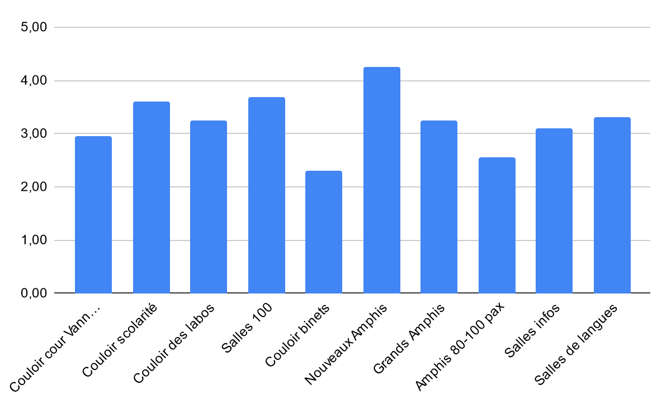
\includegraphics[width=0.9\textwidth]{images/survey_result.png}
		\caption{Survey results for Ecole Polytechnique}
	\end{figure}
\end{minipage}
\begin{minipage}{0.4\textwidth}
	The rooms were divided into 10 types, based on their location, equipment, and capacity. The survey was sent out to 70 students, 33 of which responded. At Ecole Polytechnique,
	rooms in the same corridors (or wing) have the same equipment and roughly the same size, leading to an easy grouping of the rooms into types.

	The results show that students have clear preferences for certain room types, as grading of the rooms varies between 2.2 to 4.1 out of five. With the results grouped around 3, the standard deviation is quite low.
	This implies that preferences exist but as $\text{average} - \text{standard deviation} < 1$, they are not too strong. Therefore, not having your top choice while not
	ideal would not be a game-breaking issue. In conclusion, this means that a classroom allocation optimization is warranted\\
\end{minipage}

These preferences are driven by four major differentiation factors that play a role in the learning experience and the quality of life of students and faculty. Room equipment represent the
first key driver, from screens, to boards, a good projector, the provision of enough power outlets for students, or even the tables used for the room. The second driver, room size, is critical
to accommodate the cohort, and what type of work is done in the room, which brings us to the third driver the room layout, be it inclined, flat, or very long and narrow. Finally, the proximity to
essentials such as the coffee machine, the labs of the professor, or the canteen is also a key driver, encompassed with things such as the number of stairs in our fourth driver: location and accessibility.
Overall, there are a variety of factors that affect learning and quality of life, and the preferences of both students and teachers reflect that.

\subsection{Simulated strategies for courses}

In order to test the algorithm and deliver some simulated results, the registrar's office at Ecole Polytechnique provided us with the list of the rooms and their capacities.
We did not however have the list of the courses and their cohort size, so we had to simulate this data. We used a random distribution of the cohort size, but with parameters that
simulate the difference we can have between tutorials and lectures, and the fact that some courses are more popular than others. Therefore, 85\% of the courses have a cohort size between 10 and 35,
representing tutorials (and the classes of the third years and masters which are highly specialized), while the remaining 15\% have a cohort size between 35 and 200, representing lectures.\\

Additionally, several strategies regarding the preferences of the courses were devised and tested in order to see the impact of the preferences on the final allocation, and test different
scenarios: 

\begin{itemize}
	\item \textbf{Random}: The courses have random preferences for the room types based on an uniform distribution
	\item \textbf{Smart Random}: The courses have uniform random preferences for the room types, but only if a room with sufficient capacity exists in the type.
	\item \textbf{Size-based}: The courses have preferences based on the average room size of the type, and rank them to minimize the difference between it and the cohort size.
	\item \textbf{Fixed preferences}: The courses have fixed preferences for the room types, based on the survey results (average grade). In that case all courses have the same preferences, in decreasing order of the average grade.
	\item \textbf{Satisfaction}: The courses have preferences based on the pooling of students, so as to represent a real life scenario (with extrapolation to increase the number of courses to an arbitrary number). 
	We therefore have more variation in the preferences expressed compared to the fixed preferences.
\end{itemize}

Once the strategies were defined, the algorithm was able to run on simulated data and produce results which we will detail in the next section. The other parameter that can vary is the number of preferences
expressed, from 3 to 10 (max). Unless stated otherwise, the results are based on the 76 rooms of Ecole Polytechnique,and between 65 and 70 courses, with 20 run averages for each strategy.

\subsection{Results and Analysis}

\subsubsection*{Allocation rate by strategy}

The graph below shows the allocation rate for each strategy, with the number of preferences expressed (3, 5 or 10). The allocation rate is defined as the percentage of courses that have been
allocated a room at the end of the process.\\

The Fixed (fixed\_10) and Smart Random (smart\_random\_10) strategies have the highest allocation rates, at 99.7\%, where courses are all allocated a room, except for rare cases where there are
too many big courses simultaneously. This is to be expected as courses run through all the room types, and therefore have a near 100\% chance of being allocated a room. The fixed strategy is our
worst-case scenario, as it represents a scenario where all courses have the same preferences, and the algorithm has to allocate them based on the capacity of the rooms, and a lot of shuffling is needed.

\begin{minipage}{0.55\textwidth}
	\begin{figure}[H]
		\centering
		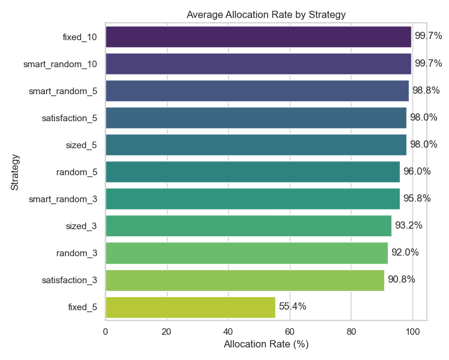
\includegraphics[width=0.9\textwidth]{images/allocation_rate.png}
		\caption{Average Allocation rate over 20 runs by strategy and number of preferences}
	\end{figure}
\end{minipage}
\hfill
\begin{minipage}{0.4\textwidth}
	The theoretical best-case scenario, Size-based (sized\_3 and sized\_5) where the courses have preferences based on expected room capacity, meaning rooms with capacities closest to the cohort size, performs
	well even at low preference numbers. The Smart Random strategy, where the courses have random preferences but only if a room with sufficient capacity exists in the type, also performs well at 98.8\%,
	explained by the rooms having spread-out preferences, with no "dead-end" room types that would be too small for them.\\

	The real life scenario (satisfaction\_5), performs well at 98\%, indicating that when using real life preferences based on student polling, the algorithm can still achieve high allocation rates.\\
\end{minipage}
\linebreak

This is particularly important as it represents the most realistic scenario among all tested strategies. It also indicates that ranking all 10 room types would not be necessary, as 98\% of the
courses are already allocated using 5 preferences.

One conclusion that can be drawn from this graph is the importance of spreading out preferences for the rooms, as varied choices allow for better allocation rates. However this cannot be done without
a variety of room types offering the basic requested features from faculty and students.

There is a clear and expected pattern, that allowing more preferences generally improves allocation rate across all strategies. Random for example improves from 92\% to 96\% with 5 preferences, which we can
explore next.

\subsubsection*{Impact of the number of preferences}

The simulations are based on the Satisfaction strategy, as it represents the most realistic scenario. The impact of the number of preferences expressed by the courses on the allocation rate is shown below. The parameters are 70 courses,
76 rooms, and a cohort size between 10 and 200, averaged over 100 runs. For each run, the seed for the random number generator is fixed to ensure coherence of the results.

\begin{minipage}{0.4\textwidth}
	The data shows that allowing more preferences consistently leads to better allocation rates, with a particularly significant improvement as they increases from 1 to 6.
	When courses can express only one preference (satisfaction\_1), the allocation rate is relatively low at 52.7\%. However, this rate improves dramatically to 78.8\% with two preferences and
	continues to rise steadily with each additional preference option.\\

	A notable threshold appears at 6 preferences, where the allocation rate reaches 99.1\%. Beyond this point, the improvements become marginal, with 7, 8, and 9 preferences all achieving nearly
	identical rates of 99.2\%. This suggests that 6 preferences may represent an optimal balance point between choosing complexity for faculty and allocation efficiency. This indicates a
	good sign of being able to allocate nearly all courses with a limited number of preferences.
\end{minipage}
\hfill
\begin{minipage}{0.55\textwidth}
	\begin{figure}[H]
		\centering
		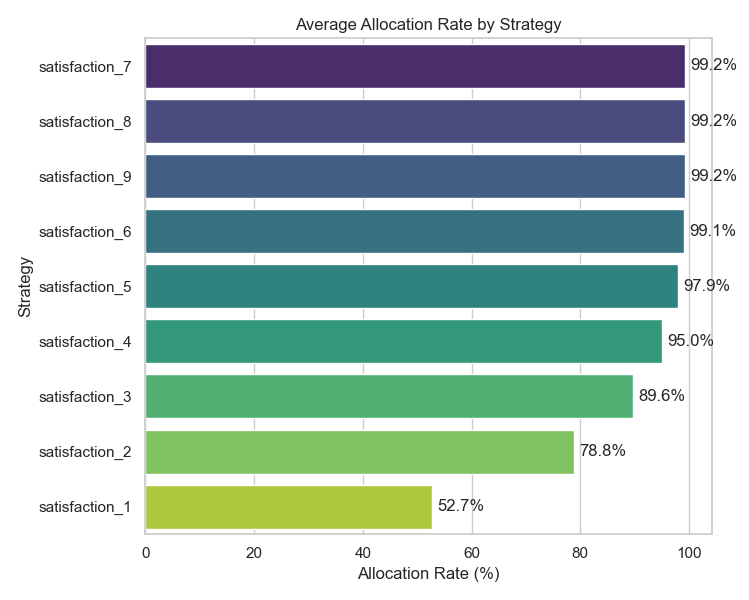
\includegraphics[width=0.9\textwidth]{images/strategy_comparison.png}
		\caption{Impact of the number of preferences on the allocation rate}
	\end{figure}
\end{minipage}

\subsubsection*{Performance and satisfaction metrics}

The efficiency of the matching process implemented in \castle{} has been measured by two key metrics: Average choice rank and high-rank rate defined as follows: Average choice rank is simply the average rank
of the room type allocated to the courses in its preferences, while the high-rank rate is the percentage of courses that have been allocated a room out of the top three. These metrics are important for the
satisfaction of the system, as they show how well the preferences of the courses are taken into account. In both cases, the lower the value, the better the performance.

\begin{figure}[H]
	\centering
	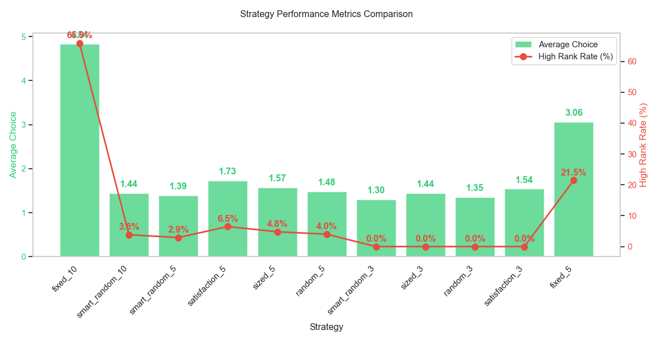
\includegraphics[scale = 0.8]{images/performance_metrics.png}
	\caption{Average choice rank and high-rank rate by strategy and number of preferences}
\end{figure}

Here we clearly see the worst cases scenario for the Fixed strategy, where the average choice rank of 4.9 and a high rank rate of 65.9\%. This is to be expected as the courses have the same preferences.
The focus here is on the other strategies, none of which go over 2 for the average choice rank, and high-rank rate under 7\%. This globally indicates that the algorithm is able to allocate the courses
to their top choices, while respecting the capacity constraints and the needs of the administration. The high-rank rate is particularly important, as it shows that there would be very few professors and 
teaching assistants that would not be satisfied with their room allocation.

The real life based scenario: satisfaction, has one of the worst performance metrics, with an average choice rank of 1.73 and a high-rank rate of 6.5\%. While not the best, this is still a very good result,
and shows what \castle{} can achieve.

\section{Effects of the \castle{} system and next steps}

\subsection{Maximum Utilization of Resources}

One of the visible effects of the \castle{} system is the maximum utilization of the most requested resources, as the algorithm is designed to minimize the difference between the cohort size and the room capacity.
This is particularly important to allow the best rooms to be used by the most students and thus get the most out of the school investment in these capacities. For the case of Ecole Polytechnique, using the
real life scenario, the top 5 room types are used at 100\%, and they have very high occupancy rate, as seen in the graph below. The lower occupancy rate for the \textit{Grands Amphis} and \textit{Nouveaux Amphis}
is due respectively to being the biggest rooms up to 800 students (while the simulation only goes up to 200 for lectures), and tutorials being simulated to 35 students max while the room can hold 50. Accounting for
those two abnormalities, the most requested rooms are used at over 80\% of their capacity, which is a very good result and shows the efficiency of the algorithm in allowing more students to benefit from the best rooms.

\begin{figure}[H]
	\centering
	\begin{subfigure}{0.32\textwidth}
		\centering
		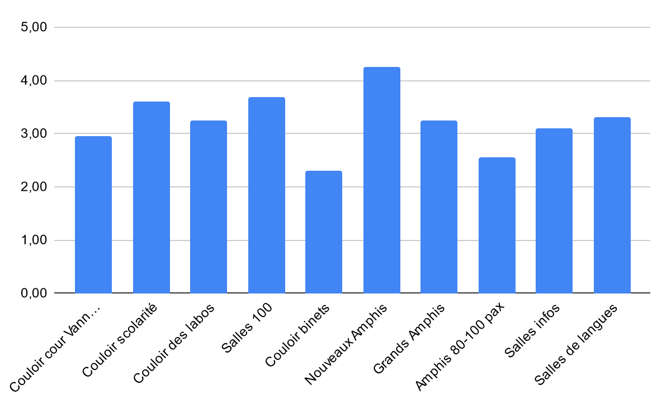
\includegraphics[width=\textwidth]{images/survey_result.png}
		\caption{Recap of the survey results}
		\label{fig:subfig1}
	\end{subfigure}
	\hfill
	\begin{subfigure}{0.65\textwidth}
		\centering
		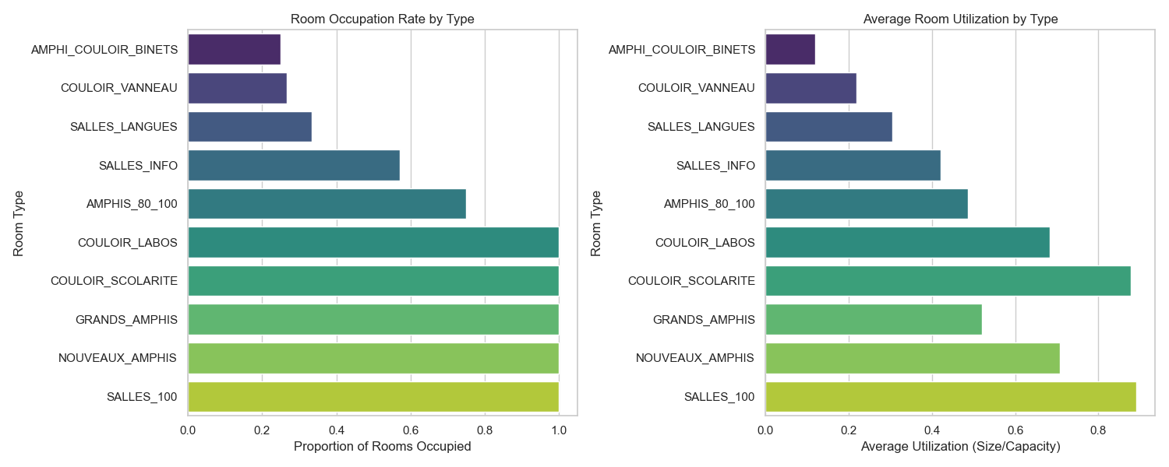
\includegraphics[width=\textwidth]{images/ressource_priority.png}
		\caption{Percentage of rooms used and occupancy rate}
		\label{fig:subfig2}
	\end{subfigure}
	\caption{Effect of signaling maximum utilization of resources}
	\label{fig:mainfig}
\end{figure}

For reference, the results of the survey are shown again in the first graph. These results show the strong correlation between the preferences from the poll and the allocation of the rooms
which is what we aim for. Less requested rooms are also used, but at lower rates, and the average occupancy is weighed down significantly by the empty rooms.

Overall, the \castle{} system allows for a better allocation of the rooms, and a better use of the resources, which is particularly important in a university setting where the number of rooms is limited.

\subsection{Quickness and modularity of the system}

As explored in the implementation section, the algorithm is very quick to run, and can be easily modified to take into account different parameters, by modifying the fit function of the rooms.
The high allocation rate ($>95\%$) and low average choice rank ($<2$)implies that the algorithm needs little to no manual intervention to account for the fringe cases where courses would end up not allocated to a room.
Moreover, the rooms in the types being ran in order of increasing capacity, which might be counter-intuitive, makes it so that any room left empty will be bigger and thus an extra course would be easier to fit in.
Most importantly, the Deferred Acceptance algorithm is stable, so no courses would ask for a room exchange, and modifying slightly the entries of the algorithm should not change the results significantly.

If there are any fringe cases, two solutions, either the Registrar's office manually allocates that room, or if possible extend the preferences of the courses to the maximum number
of room types, which allows 100\% allocation rate if there aren't more courses than rooms. Overall, \castle{} would dramatically reduce the load on the registrar's office regarding
room allocation, and coupled with a timetable allocation system, would allow for a fully automated allocation process.

Other fit parameters for example could include:
\begin{itemize}
	\item The distance from the professor's department, which makes stability harder to achieve, but improves practical aspects
	\item Rigorous equipment matching, which leads to losing strategy-proofness, and more unmatched courses, but is necessary for some subjects like computer science
	\item A long-term fairness parameter, where ties in the capacity would be broken by favoring the course that had the worse room rank in the previous allocation,
	      this would also lose strategy-proofness, but would allow for a better perceived long-term impact.
\end{itemize}

Overall, the system is very modular and can be easily adapted to the needs of the university, and the preferences of the faculty and students. Its quickness and efficiency
would allow for a quick and easy allocation process, and the stability of the algorithm would allow for a long-term deployment.\\

Next steps for \castle{} would be to implement the timetable allocation system, using most probably a graph coloring algorithm, and to test the system on a larger scale, with more room types and courses.
The algorithm could also be complemented by a front-end interface, where faculty members could input their preferences, and see the results of the allocation. This would allow for a more transparent
allocation process, and would allow for the faculty to understand the process better.
\pagebreak

\phantomsection
\section*{Conclusion}
\addcontentsline{toc}{section}{Conclusion}

The Capacity-Aligned Stable Teaching Location Engine (\castle{}) represents an advancement in addressing the complex challenge of classroom allocation in higher education institutions.
Through careful market design principles and algorithmic implementation,it achieves several critical objectives that current manual systems struggle to meet.\\

The system's core strength lies in its balance of theoretical guarantees with practical applicability.
The modified Deferred Acceptance algorithm ensures stability and Pareto efficiency, while maintaining limited manipulability (and thus relative strategy-proofness)
from faculty- properties that are essential for a long-term deployment in university settings.\\

These theoretical foundations are complemented by empirical evidence
from simulations using real preference data from Ecole Polytechnique, demonstrating consistent allocation rates above 95\% with an average choice rank below 2,
even with limited preference expression.\\

Additionally \castle{}'s computational structure, achieving O(C·R) average-case complexity, enables real-time allocation adjustments while handling the scale of modern universities.
It's modularity allows the administration to customize it with different fit functions, accommodating institution-specific priorities.
This flexibility, combined with its ability to maximize resource utilization of highly-demanded rooms, addresses the growing challenges
faced by universities, as they expand their program offerings and student populations.\\

Finally, the room allocation process is transformed from an opaque, manual task into a transparent, automated preference-based system that captures and responds to stakeholder needs.
Surveys at Ecole Polytechnique demonstrate preferences exist among faculty and students, and that these can be incorporated into the allocation process while maintaining high efficiency.
This represents a significant improvement over current systems, which often rely on single criteria like capacity or require extensive manual coordination.\\

In the future as universities continue to face pressure on their physical resources or expand, using systems like \castle{} will prove necessary.
While further developments in areas such as timetable integration and user interface design would enhance its practical implementation,
already provides a robust theoretical foundation for more efficient and satisfying classroom allocation in higher education institutions.\\

\end{document}